% Options for packages loaded elsewhere
\PassOptionsToPackage{unicode}{hyperref}
\PassOptionsToPackage{hyphens}{url}
\PassOptionsToPackage{dvipsnames,svgnames,x11names}{xcolor}
%
\documentclass[
  letterpaper,
  DIV=11,
  numbers=noendperiod]{scrartcl}

\usepackage{amsmath,amssymb}
\usepackage{iftex}
\ifPDFTeX
  \usepackage[T1]{fontenc}
  \usepackage[utf8]{inputenc}
  \usepackage{textcomp} % provide euro and other symbols
\else % if luatex or xetex
  \usepackage{unicode-math}
  \defaultfontfeatures{Scale=MatchLowercase}
  \defaultfontfeatures[\rmfamily]{Ligatures=TeX,Scale=1}
\fi
\usepackage{lmodern}
\ifPDFTeX\else  
    % xetex/luatex font selection
\fi
% Use upquote if available, for straight quotes in verbatim environments
\IfFileExists{upquote.sty}{\usepackage{upquote}}{}
\IfFileExists{microtype.sty}{% use microtype if available
  \usepackage[]{microtype}
  \UseMicrotypeSet[protrusion]{basicmath} % disable protrusion for tt fonts
}{}
\makeatletter
\@ifundefined{KOMAClassName}{% if non-KOMA class
  \IfFileExists{parskip.sty}{%
    \usepackage{parskip}
  }{% else
    \setlength{\parindent}{0pt}
    \setlength{\parskip}{6pt plus 2pt minus 1pt}}
}{% if KOMA class
  \KOMAoptions{parskip=half}}
\makeatother
\usepackage{xcolor}
\setlength{\emergencystretch}{3em} % prevent overfull lines
\setcounter{secnumdepth}{-\maxdimen} % remove section numbering
% Make \paragraph and \subparagraph free-standing
\ifx\paragraph\undefined\else
  \let\oldparagraph\paragraph
  \renewcommand{\paragraph}[1]{\oldparagraph{#1}\mbox{}}
\fi
\ifx\subparagraph\undefined\else
  \let\oldsubparagraph\subparagraph
  \renewcommand{\subparagraph}[1]{\oldsubparagraph{#1}\mbox{}}
\fi


\providecommand{\tightlist}{%
  \setlength{\itemsep}{0pt}\setlength{\parskip}{0pt}}\usepackage{longtable,booktabs,array}
\usepackage{calc} % for calculating minipage widths
% Correct order of tables after \paragraph or \subparagraph
\usepackage{etoolbox}
\makeatletter
\patchcmd\longtable{\par}{\if@noskipsec\mbox{}\fi\par}{}{}
\makeatother
% Allow footnotes in longtable head/foot
\IfFileExists{footnotehyper.sty}{\usepackage{footnotehyper}}{\usepackage{footnote}}
\makesavenoteenv{longtable}
\usepackage{graphicx}
\makeatletter
\def\maxwidth{\ifdim\Gin@nat@width>\linewidth\linewidth\else\Gin@nat@width\fi}
\def\maxheight{\ifdim\Gin@nat@height>\textheight\textheight\else\Gin@nat@height\fi}
\makeatother
% Scale images if necessary, so that they will not overflow the page
% margins by default, and it is still possible to overwrite the defaults
% using explicit options in \includegraphics[width, height, ...]{}
\setkeys{Gin}{width=\maxwidth,height=\maxheight,keepaspectratio}
% Set default figure placement to htbp
\makeatletter
\def\fps@figure{htbp}
\makeatother

\KOMAoption{captions}{tableheading}
\makeatletter
\makeatother
\makeatletter
\makeatother
\makeatletter
\@ifpackageloaded{caption}{}{\usepackage{caption}}
\AtBeginDocument{%
\ifdefined\contentsname
  \renewcommand*\contentsname{Table of contents}
\else
  \newcommand\contentsname{Table of contents}
\fi
\ifdefined\listfigurename
  \renewcommand*\listfigurename{List of Figures}
\else
  \newcommand\listfigurename{List of Figures}
\fi
\ifdefined\listtablename
  \renewcommand*\listtablename{List of Tables}
\else
  \newcommand\listtablename{List of Tables}
\fi
\ifdefined\figurename
  \renewcommand*\figurename{Figure}
\else
  \newcommand\figurename{Figure}
\fi
\ifdefined\tablename
  \renewcommand*\tablename{Table}
\else
  \newcommand\tablename{Table}
\fi
}
\@ifpackageloaded{float}{}{\usepackage{float}}
\floatstyle{ruled}
\@ifundefined{c@chapter}{\newfloat{codelisting}{h}{lop}}{\newfloat{codelisting}{h}{lop}[chapter]}
\floatname{codelisting}{Listing}
\newcommand*\listoflistings{\listof{codelisting}{List of Listings}}
\makeatother
\makeatletter
\@ifpackageloaded{caption}{}{\usepackage{caption}}
\@ifpackageloaded{subcaption}{}{\usepackage{subcaption}}
\makeatother
\makeatletter
\@ifpackageloaded{tcolorbox}{}{\usepackage[skins,breakable]{tcolorbox}}
\makeatother
\makeatletter
\@ifundefined{shadecolor}{\definecolor{shadecolor}{rgb}{.97, .97, .97}}
\makeatother
\makeatletter
\makeatother
\makeatletter
\makeatother
\ifLuaTeX
  \usepackage{selnolig}  % disable illegal ligatures
\fi
\IfFileExists{bookmark.sty}{\usepackage{bookmark}}{\usepackage{hyperref}}
\IfFileExists{xurl.sty}{\usepackage{xurl}}{} % add URL line breaks if available
\urlstyle{same} % disable monospaced font for URLs
\hypersetup{
  pdftitle={AI's Evolution in Manufacturing: Shaping Jobs and the Workforce of Tomorrow.},
  pdfauthor={Alex Paul Kelly},
  colorlinks=true,
  linkcolor={blue},
  filecolor={Maroon},
  citecolor={Blue},
  urlcolor={Blue},
  pdfcreator={LaTeX via pandoc}}

\title{AI's Evolution in Manufacturing: Shaping Jobs and the Workforce
of Tomorrow.}
\author{Alex Paul Kelly}
\date{2024-12-07}

\begin{document}
\maketitle
\ifdefined\Shaded\renewenvironment{Shaded}{\begin{tcolorbox}[breakable, boxrule=0pt, sharp corners, interior hidden, frame hidden, borderline west={3pt}{0pt}{shadecolor}, enhanced]}{\end{tcolorbox}}\fi

\renewcommand*\contentsname{Table of contents}
{
\hypersetup{linkcolor=}
\setcounter{tocdepth}{4}
\tableofcontents
}
\hypertarget{overview}{%
\section{Overview}\label{overview}}

\href{https://www.makeuk.org/insights/publications/uk-manufacturing-the-facts-2023\#/}{Manufacturing
is a key sector for the UK economy, accounting for 10\% of GDP and 44\%
of exports, the UK is the 8th largest exporter in the world}.
Manufacturing didnt use to be about computing technology. It was about
the materials and the processes. Computing and data is now at the centre
and key to the future of manufacturing. This article will explore the
impact of AI on manufacturing jobs, and how this will affect the
workforce. It will also look at what roles will be created in the
future, and how these roles will will help the uk manufacturing sector.
This will indicate how manufacturing will look in the future.

\hypertarget{evolution-of-manufacturing-3rd-4th-5th-industrial-revolutions}{%
\section{Evolution of manufacturing : 3rd, 4th, 5th industrial
revolutions}\label{evolution-of-manufacturing-3rd-4th-5th-industrial-revolutions}}

\begin{figure}

{\centering 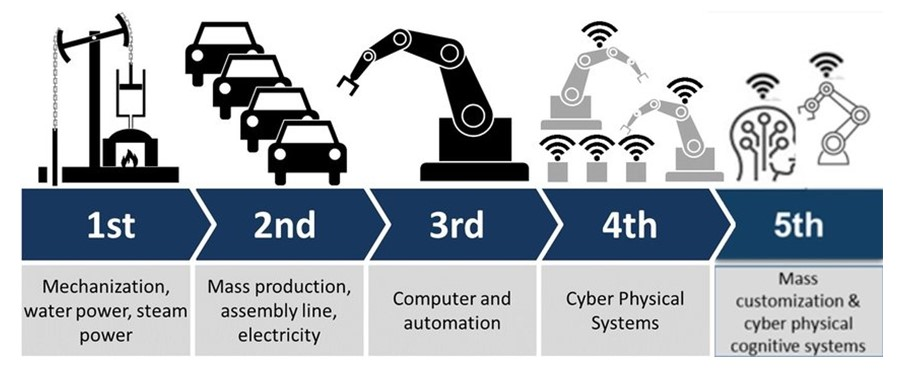
\includegraphics{./Industry5.jpg}

}

\caption{picture of industrial revolutions}

\end{figure}

You can see from the image above,computers started to appear in:

The \textbf{3rd industrial revolution} but there were lots of companies
that didnt have IT systems and when they did, they were not joined up.
The IT systems were maybe stock control, accounting, or an ERP system
and PLC's to automate machines that were previously manual.

The \textbf{4th industrial revolution} the IT systems are more joined up
and the machines and parts and factories make use of IOT (internet of
things) systems. All this allows for real-time data exchange and
monitoring. This connectivity facilitates more efficient operations,
predictive maintenance, and improved decision-making based on
comprehensive data analysis. This is where most manufacturing companies
are now but some are remecent to change and are still in the 3rd
industrial revolution.

The \textbf{5th industrial revolution} While still largely conceptual
and not universally recognized as a distinct phase, the idea of a fifth
industrial revolution often revolves around the integration of advanced
technologies like AI and robotics into the manufacturing process. This
could lead to even greater automation, with AI making complex decisions
and managing processes. The focus is not just on efficiency and
productivity but also on personalization and sustainability. The impact
on economies and workforces would be significant, as it would
necessitate a shift in skills and roles.

\hypertarget{the-current-state-of-ai-in-manufacturing}{%
\section{The Current State of AI in
Manufacturing}\label{the-current-state-of-ai-in-manufacturing}}

AI is already being used in manufacturing, but it's still in its
infancy. The majority of AI applications in manufacturing are focused on
improving efficiency and productivity. This includes predictive
maintenance, supply chain optimization, and process automation. There
are a lot of classification models for quality but more growth will be
on the generative models. The impact of AI on manufacturing is expected
to grow significantly in the coming years, with the global market for
\href{https://www.businesswire.com/news/home/20221103005709/en/16.3-Billion-Worldwide-Artificial-Intelligence-in-Manufacturing-Industry-to-2027---Featuring-Bright-Machines-Cisco-Systems-Flutura-and-General-Vision-Among-Others---ResearchAndMarkets.com}{AI
in manufacturing projected to reach \$16.7 billion by 2026}.

\hypertarget{personal-experience-ais-impact-on-my-workflow}{%
\subsection{Personal Experience: AI's Impact on My
Workflow}\label{personal-experience-ais-impact-on-my-workflow}}

As a IT worker in manufacturing, my work flow has change due to the
advancements in AI. I'm a ahead of the rest of the business in terms of
using AI to improve my workflow and results it gives to the business.

I use to speak to the the people in business (my customers),
understanding their/the businesses requirements, and then building a
solution and iterate between the two and maybe use a 3rd party for extra
resources to finish the solution in a quicker time.

The approach I use has evolved. While I still communicate with
colleagues, I now employ AI and data science techniques to extract and
organize information from various structured and unstructured systems.
This allows me to present data to the business in a more efficient and
effective manner. Prior to recent technological advancements, managing
this process alone wouldn't have been cost-effective. Currently, I
leverage these tools to distill information, which aids in making
decisions or uncovering additional insights and requirements.

When a solution is required, I'm now using AI to help me build the
solution in record time and with better quality, giving the business a
better return on their investment in me, affectivly increasing my worth.
The AI models I'm using are general purpose models that have been
trained on lots of data but im using them to build unique products and
solutions that are a fit for our business. Building solutions using AI
and building on existing foundation AI models is the future of
manufacturing.

Other people in the business will improve their work flow by using
generalized AI models and systems to help them make decisions and
automate processes their own processes. They will also get the benefit
of the work I'm doing (IT department), as I am be able to build
solutions to improve their processes.

This will free up their time to do more value added work. This will
increase their worth to the business. This will increase the UK economy.
This will increase the UK productivity.

\hypertarget{the-economics-of-ai-in-manufacturing}{%
\subsection{The Economics of AI in
Manufacturing}\label{the-economics-of-ai-in-manufacturing}}

Graphics cards (tensor procceses) are the hardware that compute AI
models. The sale of these cards gives a great insight into the future
demand of AI, it's one of the limiting factors in more models and end
users using those models. GPU demand is outstripping supply and is
likley to do for a long time. Companies are racing to train the latest
models, updating existing models and providing compute for inference
(querying models for results). All of this requires more GPU's. Here's
some stats from {[}GPU economics{]}
(https://www.latent.space/p/semianalysis) on the growth of GPU's:

\begin{itemize}
\tightlist
\item
  NVIDIA is forecasted to sell over 3 million GPUs next year, about 3x
  their 2023 sales of about 1 million H100s.
\item
  AMD is forecasting \$2B of sales for their new MI300X datacenter GPU.
  They are also indirectly getting a boost from the work that companies
  like Modular and tiny are doing in making it easier to actually use
  these chips (will ROCm ever catch up?).
\item
  Google's TPUv5 supply is going to increase rapidly going into 2024.
\item
  Microsoft just announced Maia 100, a new AI accelerator built ``with
  feedback'' from OpenAI. and much more.
\end{itemize}

Having more compute will increase competition and drive down prices.
This will allow more companies to use AI and more people to use AI. This
will increase the demand for AI and the demand for AI workers.

\hypertarget{software-evolution-from-1.0-to-3.0-in-manufacturing}{%
\section{Software Evolution: From 1.0 to 3.0 in
Manufacturing}\label{software-evolution-from-1.0-to-3.0-in-manufacturing}}

Software is changing, the pace of change is accelerating due to AI. The
future of software is going to be very different to the past. Software
is at the heart of manufacturing, it's used to control the machines,
it's used to control the processes, it's used to control the supply
chain, it's used to understand the business and help control the
business. Manufactures leadership and employees need to be aware of
these changes and secondly, they are going to need to adapt to this
change. They need to realise that this change is key to the 4th and 5th
industrial revolutions mentioned above and their future success. The
manufactures that adapt the quickest will be the ones that profit and
grow. The manufactures that don't adapt will be left behind. Now a
little about the software evolution.

\begin{itemize}
\tightlist
\item
  Software 1.0: Hand-coded software with conditional logic, loops, etc.
\end{itemize}

The deterministic nature of Software 1.0 made it highly reliable and
predictable, which was crucial for manufacturing processes where
precision and consistency were non-negotiable. However, this method had
its limitations. It was labor-intensive and less adaptable, requiring
substantial human effort for updates and modifications.

\begin{itemize}
\tightlist
\item
  Software 2.0: Machine learning models like neural nets trained on data
\end{itemize}

Software 2.0 signifies a paradigm shift towards machine learning models,
particularly neural networks. Instead of manually programming every
possible outcome, this era focused on training models on large datasets.
These models could then learn patterns, make decisions, and adapt to new
data, making them more flexible than their predecessors.

\begin{itemize}
\tightlist
\item
  Software 3.0: Using large pre-trained foundation models without
  needing to collect/label training data
\end{itemize}

Software 3.0 is where the future begins to unfold, characterized by the
use of large, pre-trained foundation models. These AI models, having
been trained on extensive, diverse datasets, can be fine-tuned for
specific tasks, drastically reducing the need for new data collection
and labeling.

There will be a transition between software 2 and 3. We're in a weird
space where alot of people/companies are still in software 1.0 and
trying out features from software 2.0 but also using 3.0 on occation. i
think all 3 will exist for a long time but will be seeing more growth in
software 2.0 and espeicllay 3.0.

\hypertarget{the-future-of-manufacturing-software}{%
\subsection{The Future of Manufacturing
Software}\label{the-future-of-manufacturing-software}}

In the manufacturing sector, Software 3.0 opens up new horizons. It
allows for greater customization, efficiency in processes, and enhanced
predictive capabilities for maintenance and supply chain management. The
integration of AI with IoT and robotics leads to smarter, more connected
factories.

\hypertarget{democratization-of-advanced-machine-learning-technologies-in-manufacturing}{%
\subsection{Democratization of Advanced Machine Learning Technologies in
Manufacturing}\label{democratization-of-advanced-machine-learning-technologies-in-manufacturing}}

The democratization of AI is a key driver of this evolution. The
availability of foundation models and the ease of use of AI platforms
are lowering the barrier to entry. This is enabling more people to
leverage AI in their work, including those without extensive data
science expertise. The result is a shift in the role of software
engineers, from building models to consuming them. This is the rise of
the AI engineer.

\hypertarget{what-will-new-ai-roles-look-like}{%
\section{What will new AI roles look
like}\label{what-will-new-ai-roles-look-like}}

\hypertarget{over-view}{%
\subsection{Over view}\label{over-view}}

It use to be that you needed expert maths skills , data science and
coding skills to be able to build and train models and then a lot of
experience in all of the roles. You would need to know how to prepare
data, how to train models, how to evaluate models, how to deploy models,
how to monitor models, how to retrain models, how to update models, how
to use models. You would need indepth knowledge of them all or more
likely, be in a team where have, a data prepartion expert, an expert in
models for the different types of data, and architecture to be able to
comunicate between these roles and many more roles. A lot of the tooling
improvements have enabled this to be done by one person or a very small
team depending on how big the project is.

The most talked about model is chatgpt. Its a chatbot inferface where
you ask questions (prompt) and it will give you an answer. There are
other less known models where you just ask what you want in text and it
return in other forms such as images, text, video, audio, 3d modles.
Anyone who can use a computer can use these models. All it takes is
understanding what models are available, what they do for you and how to
get the best outputs for your inputs. This will be a key skills to have.

For more advance users/developers there are more specific solutions for
producing code within a development enviroment like microsoft copilot
offers. There are over 15,000 off the shelf models from huggingface
raning from nlp, multimodel, computer vision, speech processing and many
more. All these models have there weights release which means that they
can be use as is or customize (fine tuned) to your own organizational
needs, no need to start from scratch. On hugging face, there are
datasets ready to be used to train Neural network and spaces to allow
you to use the models. This is where things start to get interesting.

\hypertarget{enter-the-ai-engieer}{%
\subsection{Enter the AI engieer,}\label{enter-the-ai-engieer}}

In the rapidly evolving landscapes of Industry 4.0 and 5.0, the role of
the AI engineer emerges as a pivotal element. This role is defined by a
deep understanding of the problem domain, comprehensive knowledge of AI
models and ecosystems, and the ability to apply this expertise to
deliver tangible business outcomes. These outcomes can range from
gaining new insights and automating tasks, to enhancing the quality of
products. The AI engineer leverages the principles of what can be
described as ``software 3.0'' but can include software 1.0 and 2.0. Some
specific applications of AI in manufacturing include:

\begin{itemize}
\tightlist
\item
  Predictive Maintenance: A car manufacturing company uses AI algorithms
  to analyze data from assembly line robots. The AI predicts when a
  robot's components are likely to fail, allowing for maintenance before
  a breakdown occurs, thereby reducing production downtime.
\item
  Supply Chain Optimization: A consumer electronics manufacturer employs
  AI to forecast demand for its products, adjusting production schedules
  and inventory levels accordingly. This AI-driven approach helps the
  company avoid overproduction and stock shortages.
\item
  Personalized Manufacturing: A furniture company uses AI to offer
  customers the ability to customize products online. The AI assists in
  translating these customizations into manufacturing instructions,
  enabling mass customization at scale.
\item
  Energy Efficiency: A steel plant uses AI to optimize its furnaces'
  energy consumption. The AI system constantly analyzes production data
  and adjusts furnace operations to maximize energy efficiency while
  maintaining quality.
\item
  Quality Control: A pharmaceutical company implements AI for real-time
  quality control. The AI system continuously analyzes images of drug
  capsules to identify and sort out defects, ensuring high-quality
  products.
\item
  Worker Safety and Ergonomics: An AI system in a chemical plant
  monitors the workplace environment using sensors and cameras. It
  identifies potential safety hazards and suggests ergonomic
  improvements to reduce the risk of worker injuries.
\item
  Process Optimization: In a textile factory, AI algorithms analyze the
  entire production process, identifying bottlenecks and suggesting
  improvements to enhance throughput and reduce waste.
\item
  Market Analysis and Consumer Insights: An AI system helps a toy
  manufacturer analyze social media trends and consumer feedback to
  predict which toy designs are likely to be popular, guiding product
  development and marketing strategies.
\item
  Collaborative Robotics (Cobots): In a packaging facility, cobots
  equipped with AI work alongside human employees, taking over
  repetitive tasks and reducing the physical strain on workers.
\item
  Customized AI Solutions: A bespoke AI solution is developed for a food
  processing company to monitor and optimize the ripening process of
  fruits, enhancing product quality.
\item
  Training and Simulation: AI-driven virtual reality simulations are
  used in an aerospace company to train assembly workers, reducing the
  learning curve and improving precision in complex tasks on high value
  products. This helps to reduce the cost of training and the cost of
  mistakes.
\item
  Environmental Monitoring and Compliance: An AI system in a cement
  factory monitors emissions in real-time, ensuring compliance with
  environmental regulations and identifying areas for improvement.
\item
  Enhancing Customer Experiences: An AI chatbot in a manufacturing
  company's customer service department provides quick and accurate
  responses to customer inquiries, improving satisfaction.
\item
  Integrating IoT with AI: In a smart factory, AI algorithms analyze
  data from IoT sensors
\end{itemize}

Foundation models like GPT-3/4, Claude, and Whisper, signify a shift in
the AI paradigm. These models are accessible off-the-shelf via APIs,
offering a streamlined path to implementation. Understanding the
architecture of these models - their layers and structure - is crucial.
The ability to employ a pre-trained model bypasses the need for
extensive data collection and training, accelerating the deployment
process.

Putting these foundation models into production varies in complexity. It
can be as simple as calling an API where no knowledge of infrastrucure
is required. Or as intricate as running the models locally, serving
high-volume predictions. Running locally and managing demands requires a
keen understanding of GPU utilization, batching, and infrastructure
expertise.

The emergence of AI engineers is reshaping the landscape of development.
AI is becoming increasingly accessible to traditional software
engineers, blurring the lines between machine learning engineers and AI
engineers. The latter focuses more on consuming foundation model APIs
and the former more on building models from scratch.

This shift has economic implications. The demand for AI far exceeds the
supply of machine learning experts. Consequently, AI engineers are
evolving from software engineers who acquire these specialized skills.

The AI engineering stack is defined by systems of reasoning and
retrieval-augmented generation stacks. These connect models to diverse
data sources, broadening the scope of application.

AI UX is expanding beyond chatbots, introducing new modalities and
interfaces. Building products with these foundation models requires a
focus on delivering unique value, solving customer problems, and
building trust.

However, there's a balance to be struck. While some skepticism towards
AI is healthy, there's also a tendency to unfairly blame AI for
shortcomings. The hype generated by media and industry creators sets
high expectations. It's essential for AI engineers to remain grounded in
real customer needs.

The impact of AI applications is already being felt in various sectors,
demonstrating the positive influence of these technologies. For AI
engineers, this era represents an unprecedented opportunity to innovate,
explore, and shape the future of industries 4.0 and 5.0. Their role is
not just about technical proficiency, but also about envisioning and
realizing the potential of AI to transform industries and improve lives.

\href{https://www.latent.space/p/aies-podrocket}{Rise of the AI
engineer}



\end{document}
